% Grundlagen
\chapter{Grundlagen}

\section{Grundsätzliche Arbeitsweise eines Simulators}

Ein Simulator ist eine Software, welche das Verhalten eines realen Systems nachbildet. Im Fall eines Mikrocontrollers wie dem PIC wird die Hardwarearchitektur – bestehend aus Central Processing Unit (CPU), Speicher, Registern und Peripheriekomponenten – virtuell nachgebildet, um Programme auszuführen, als würden sie auf der physischen Hardware laufen. Die grundsätzliche Arbeitsweise eines solchen Simulators umfasst typischerweise die folgenden, eng miteinander verzahnten Schritte:

\begin{itemize}
    \item \textbf{Laden des Programms}: Der erste Schritt besteht darin, das zu testende Programm in den simulierten Speicher des Mikrocontrollers zu laden. Dieses Programm liegt üblicherweise in einem maschinenlesbaren Format vor, oft als Ergebnis eines Assemblierungs- oder Kompilierungsvorgangs (z.B. eine .LST-Datei, die sowohl den Maschinencode als auch die ursprünglichen Assemblerinstruktionen enthält, oder eine .HEX-Datei). Der Simulator liest diese Datei ein, interpretiert die enthaltenen Daten und platziert die Programmanweisungen und initialen Datenwerte an den entsprechenden Stellen im simulierten Programmspeicher und Datenspeicher.
    \item \textbf{Dekodieren der Instruktionen}: Nachdem das Programm geladen ist, beginnt der Simulator mit der Ausführung. Dazu liest die simulierte CPU die erste Instruktion aus dem Programmspeicher, auf die der Programmzähler (Program Counter, PC) zeigt. Jede dieser Instruktionen ist ein binärer Code, der vom Simulator dekodiert werden muss. Das Dekodieren bedeutet, den binären Code zu analysieren, um festzustellen, welcher spezifische Befehl (z.B. Addition, Datenverschiebung, Sprungbefehl) ausgeführt werden soll und welche Operanden (z.B. Register, Speicheradressen, konstante Werte) dafür benötigt werden.
    \item \textbf{Ausführen der Instruktionen}: Nach der Dekodierung führt die simulierte CPU die entsprechende Operation aus. Dies beinhaltet die Manipulation von Daten in den simulierten Registern, das Lesen oder Schreiben von Werten im simulierten Speicher und die Aktualisierung von Statusregistern (Flags), wie z.B. dem Zero-Flag, Carry-Flag oder Overflow-Flag, basierend auf dem Ergebnis der Operation. Der Simulator muss das Verhalten jeder einzelnen Instruktion des Ziel-Mikrocontrollers exakt nachbilden. Nach der Ausführung einer Instruktion wird der Programmzähler in der Regel inkrementiert, um auf die nächste Instruktion zu zeigen, es sei denn, es wurde ein Sprung- oder Verzweigungsbefehl ausgeführt.
    \item \textbf{Interaktion mit Peripherie}: Moderne Mikrocontroller verfügen über eine Vielzahl von integrierten Peripheriegeräten wie Timer/Counter, Interrupt-Controller, serielle Schnittstellen (UART, SPI, I2C), Analog-Digital-Wandler (ADC) und digitale Ein-/Ausgabe-Ports (I/O-Ports). Wenn das Programm mit diesen Peripheriegeräten interagiert (z.B. einen Timer startet, einen Wert von einem I/O-Port liest oder einen Interrupt auslöst), muss der Simulator dieses Verhalten ebenfalls nachbilden. Dies kann bedeuten, interne Zustände der simulierten Peripherie zu ändern, simulierte Zeitabläufe zu verwalten oder externe Ereignisse (z.B. ein simuliertes Signal an einem I/O-Pin) zu verarbeiten.
    \item \textbf{Visualisierung und Debugging-Unterstützung}: Ein wesentlicher Aspekt vieler Simulatoren ist die Fähigkeit, den internen Zustand des simulierten Systems dem Benutzer darzustellen. Dies umfasst die Anzeige der aktuellen Werte von CPU-Registern, Speicherinhalten, dem Zustand von Peripheriegeräten und Flags. Viele Simulatoren bieten darüber hinaus erweiterte Debugging-Funktionen an, wie das Setzen von Haltepunkten (Breakpoints), schrittweise Ausführung des Programms (Single-Stepping), das Verfolgen von Variablenwerten und die Möglichkeit, Register- und Speicherwerte während der Simulation manuell zu ändern. Diese Visualisierung und Interaktion machen den Programmablauf transparent und erleichtern die Fehlersuche erheblich.
\end{itemize}

\section{Vor- und Nachteile einer Simulation}

Simulationen bieten zahlreiche Vorteile für den Entwicklungsprozess von Embedded Systems, bringen jedoch auch spezifische Einschränkungen mit sich, die berücksichtigt werden müssen.

\subsection*{Vorteile}
\begin{itemize}
    \item \textbf{Kosteneffizienz}: Einer der größten Vorteile ist die erhebliche Reduktion der Kosten. Es entfallen Ausgaben für die Anschaffung teurer Entwicklungsboards, spezifischer Messgeräte oder Prototypen-Hardware. Auch Kosten für Reparatur oder Ersatz bei Beschädigung durch fehlerhafte Programme oder Experimente entfallen. Dies ermöglicht insbesondere kleineren Teams oder Einzelentwicklern den Zugang zu Entwicklungswerkzeugen.
    \item \textbf{Flexibilität und schnelle Iteration}: Änderungen am Programmcode oder an der simulierten Hardwarekonfiguration, wie beispielsweise die Taktfrequenz oder der angeschlossene Peripherieumfang, können softwareseitig schnell und ohne physischen Umbau vorgenommen werden. Dies beschleunigt den Entwicklungszyklus erheblich, da verschiedene Szenarien und Konfigurationen in kurzer Zeit getestet werden können.
    \item \textbf{Umfassende Debugging-Möglichkeiten}: Simulatoren bieten oft weitreichendere Einblicke in das Systemverhalten als dies mit physischer Hardware möglich wäre. Entwickler können den Programmablauf schrittweise verfolgen (Single-Stepping), Haltepunkte (Breakpoints) an beliebigen Stellen im Code setzen, den Inhalt von Registern und Speicherbereichen in Echtzeit inspizieren und modifizieren. Auch komplexe Zustände und Zeitabläufe lassen sich detailliert analysieren, was die Fehlersuche und -behebung (Debugging) signifikant erleichtert.
    \item \textbf{Sicherheit und Risikominimierung}: Kritische oder potenziell destruktive Programmzustände können in einer simulierten Umgebung gefahrlos getestet werden. Es besteht kein Risiko, reale Hardware durch fehlerhaften Code, falsche Spannungen oder Kurzschlüsse zu beschädigen. Dies ist besonders wertvoll beim Testen von Grenzfällen oder Fehlerbehandlungsroutinen.
    \item \textbf{Frühzeitige Softwareentwicklung}: Die Softwareentwicklung kann parallel zur oder sogar vor der Fertigstellung der physischen Hardware beginnen. Dies verkürzt die Gesamtentwicklungszeit (Time-to-Market) und ermöglicht eine frühere Validierung von Softwarekonzepten.
    \item \textbf{Automatisierte Tests}: Simulatoren lassen sich gut in automatisierte Testumgebungen integrieren. Testskripte können eine Vielzahl von Szenarien durchlaufen lassen und die Ergebnisse protokollieren, was die Qualitätssicherung verbessert und Regressionstests vereinfacht.
\end{itemize}

\subsection*{Nachteile}
\begin{itemize}
    \item \textbf{Eingeschränkte Genauigkeit und Realitätsnähe}: Eine Simulation ist immer eine Abstraktion der Realität. Insbesondere timing-kritisches Verhalten, analoge Komponenten oder sehr spezifische Hardwareeigenschaften (z.B. exakte Interrupt-Latenzzeiten, parasitäre Effekte, Stromverbrauch) können oft nur angenähert oder gar nicht simuliert werden. Die Interaktion mit der realen physikalischen Umgebung (Sensoren, Aktoren) fehlt gänzlich oder muss durch Modelle nachgebildet werden.
    \item \textbf{Leistungsanforderungen an den Host-Rechner}: Die Emulation von Hardware in Software kann rechenintensiv sein, besonders bei komplexen Mikrocontrollern oder wenn die Simulation in Echtzeit oder annähernder Echtzeit erfolgen soll. Dies kann leistungsfähige Computer erfordern, um akzeptable Simulationsgeschwindigkeiten zu erreichen. Langsame Simulationen können den Entwicklungsprozess wiederum verlangsamen.
    \item \textbf{Abweichungen zur realen Hardware}: Trotz sorgfältiger Modellierung können immer subtile Unterschiede zwischen dem Verhalten des Simulators und der realen Hardware bestehen. Dies kann an unvollständiger Dokumentation der Hardware, Vereinfachungen im Simulationsmodell oder Fehlern im Simulator selbst liegen. Code, der im Simulator einwandfrei funktioniert, kann daher auf der Zielhardware unerwartetes Verhalten zeigen.
    \item \textbf{Entwicklungs- und Wartungsaufwand für den Simulator}: Die Erstellung und Pflege eines genauen und umfassenden Simulators ist selbst ein komplexes Softwareprojekt, das Ressourcen bindet. Insbesondere bei neuen oder sehr speziellen Mikrocontrollern ist möglicherweise kein passender Simulator verfügbar oder muss erst entwickelt werden.
    \item \textbf{Fehlende haptische Erfahrung}: Das direkte Arbeiten mit der Hardware, das Anschließen von Komponenten und das Messen von Signalen vermittelt ein tieferes Verständnis für das System, das durch eine reine Simulation nicht ersetzt werden kann.
\end{itemize}
 
% Benuteroberfläche
\chapter{Benutzeroberfläche}

Die Benutzeroberfläche des PIC Simulators ist so gestaltet, dass sie eine intuitive und effiziente Nutzung ermöglicht. Im Folgenden werden die wichtigsten Elemente der Benutzeroberfläche und deren Handhabung detailliert beschrieben:

\section{Hauptfenster}
Das Hauptfenster des Simulators ist in mehrere Bereiche unterteilt, die jeweils spezifische Informationen und Funktionen bereitstellen:
\begin{itemize}
    \item \textbf{Code-Editor}: Der integrierte Code-Editor ermöglicht das Laden von Assemblerdateien. Breakpoints können durch einfaches Anklicken der Checkbox am Zeilenanfang gesetzt werden, um den Programmablauf gezielt zu analysieren.
    \item \textbf{Steuerelemente}: Buttons wie \texttt{Go} und \texttt{Reset} steuern die Programmausführung. Diese Steuerelemente sind übersichtlich angeordnet und leicht zugänglich.
    \item \textbf{Register- und Speicheranzeige}: Diese Bereiche zeigen den aktuellen Zustand der Register, Flags und des Speichers in Echtzeit an. Änderungen werden sofort visualisiert, um den Programmablauf nachvollziehbar zu machen und das Debugging zu erleichtern.
    \item \textbf{I/O-Visualisierung}: Die I/O-Pins des Mikrocontrollers werden interaktiv dargestellt. Benutzer können die Zustände der Pins durch Anklicken ändern, um verschiedene Szenarien zu simulieren. Ebenfalls wird angezeigt, ob ein Pin als Eingang oder Ausgang konfiguriert ist.
    \item \textbf{Peripheriegeräte}: Eine Übersicht der simulierten Peripheriegeräte, wie Timer und Interrupts, wird bereitgestellt. Diese Bereiche ermöglichen eine einfache Konfiguration und Überwachung der Peripheriefunktionen.
    \item \textbf{Statusbereich}: Der Statusbereich zeigt wichtige Informationen wie den aktuellen Program Counter (PC), den Stackpointer und die Ausführungszeit an.
\end{itemize}

\section{Menüleiste}
Die Menüleiste bietet Zugriff auf grundlegende Funktionen des Simulators:
\begin{itemize}
    \item \textbf{Datei}: Optionen zum Laden von Quelldateien.
    \item \textbf{Hilfe}: Zugriff auf die Dokumentation.
\end{itemize}

\section{Debugging-Tools}
Die Benutzeroberfläche enthält leistungsstarke Debugging-Tools, die die Fehlersuche erleichtern:
\begin{itemize}
    \item \textbf{Breakpoints}: Benutzer können Breakpoints setzen, um die Programmausführung an bestimmten Stellen zu pausieren und schrittweise fortzusetzen.
    \item \textbf{Speicherüberwachung}: Der Speicherinhalt kann in Echtzeit überwacht und bei Bedarf manuell geändert werden.
    \item \textbf{Registeranzeige}: Alle Register des Mikrocontrollers werden angezeigt, einschließlich ihrer aktuellen Werte. Die Register können ebenfalls manuell bearbeitet werden.
    \item \textbf{Statusflags}: Die Statusflags (z. B. Carry, Zero) werden in Echtzeit aktualisiert und angezeigt, um den aktuellen Zustand des Mikrocontrollers zu verdeutlichen.
\end{itemize}

\section{Visualisierung und Interaktivität}
Die Benutzeroberfläche bietet eine visuelle Darstellung des Mikrocontrollers und seiner Peripherie:
\begin{itemize}
    \item \textbf{Simulation von Peripheriegeräten}: Timer, Interrupts und andere Peripheriegeräte können simuliert und überwacht werden.
    \item \textbf{Echtzeit-Updates}: Änderungen im Programm oder in der Hardwarekonfiguration werden sofort in der Benutzeroberfläche reflektiert.
    \item \textbf{Interaktive Elemente}: Benutzer können direkt mit der Simulation interagieren, z. B. durch das Ändern von I/O-Pin-Zuständen.
    \item \textbf{Konfiguration}: Benutzer können die Taktfrequenz des Simulators anpassen.
\end{itemize}

\section{Zusammenfassung}
Die Benutzeroberfläche des PIC Simulators kombiniert Funktionalität und Benutzerfreundlichkeit. Sie bietet alle notwendigen Werkzeuge, um Programme effizient zu entwickeln, zu testen und zu debuggen. Durch die klare Struktur und die interaktiven Elemente wird die Arbeit mit dem Simulator erheblich erleichtert.

% Technische Details
\chapter{Technische Details und Funktionsweise}

\section{Beschreibung des Grundkonzepts}
Der Simulator bildet die Architektur des Mikrocontrollers nach, einschließlich CPU, Speicher, Register und Peripheriegeräten. Dabei werden alle Befehle des Mikrocontrollers interpretiert und ausgeführt, während der Zustand des Systems in Echtzeit visualisiert wird.

\section{Warum Python gewählt wurde}
Zur Umsetzung des Projekts wurde Python als Programmiersprache gewählt, da es mehrere Vorteile bietet:
\begin{itemize}
    \item \textbf{Einfache Syntax}: Python ermöglicht eine klare und übersichtliche Implementierung, was die Entwicklung erleichtert.
    \item \textbf{Schnelle Entwicklungszeit}: Dank der hohen Abstraktionsebene können Prototypen schnell erstellt und getestet werden.
    \item \textbf{Umfangreiche Bibliotheken}: Python bietet zahlreiche Bibliotheken, wie \texttt{PyQt} für die GUI, welche die Entwicklung beschleunigen.
    \item \textbf{Plattformunabhängigkeit}: Python-Programme können auf verschiedenen Betriebssystemen ausgeführt werden.
\end{itemize}

\section{Ausführung eines Befehlszyklus}

Der Befehlszyklus im PIC Simulator folgt einem klar strukturierten Ablauf. Zunächst wird die Assemblerdatei analysiert, und die darin enthaltenen Befehle in ein Array geladen, das als Programmspeicher dient. 

Zu Beginn eines Befehls Zyklus wird überprüft, ob sich der Mikrocontroller im Sleep-Modus befindet, die Ausführung pausiert wurde oder der aktuelle Befehl ignoriert werden soll. Anschließend wird der nächste Befehl aus dem Programmspeicher eingelesen und dekodiert. Der Programmzähler (Program Counter) wird daraufhin inkrementiert, um auf den nächsten Befehl zu zeigen. Basierend auf der Dekodierung wird die entsprechende Funktion ausgeführt, welche den Befehl implementiert und dabei alle relevanten Statusflags (z. B. Carry, Zero) setzt. Nach der Ausführung des Befehls wird die Laufzeit des Programms entsprechend der Befehlslänge inkrementiert. Gleichzeitig wird der Watchdog-Timer erhöht, um dessen Überwachung zu simulieren. Zum Abschluss eines Zyklus werden anstehende Interrupts geprüft und verarbeitet. Schließlich wird die Benutzeroberfläche aktualisiert, um den aktuellen Zustand des Mikrocontrollers visuell darzustellen.

\begin{figure}[H]
    \centering
    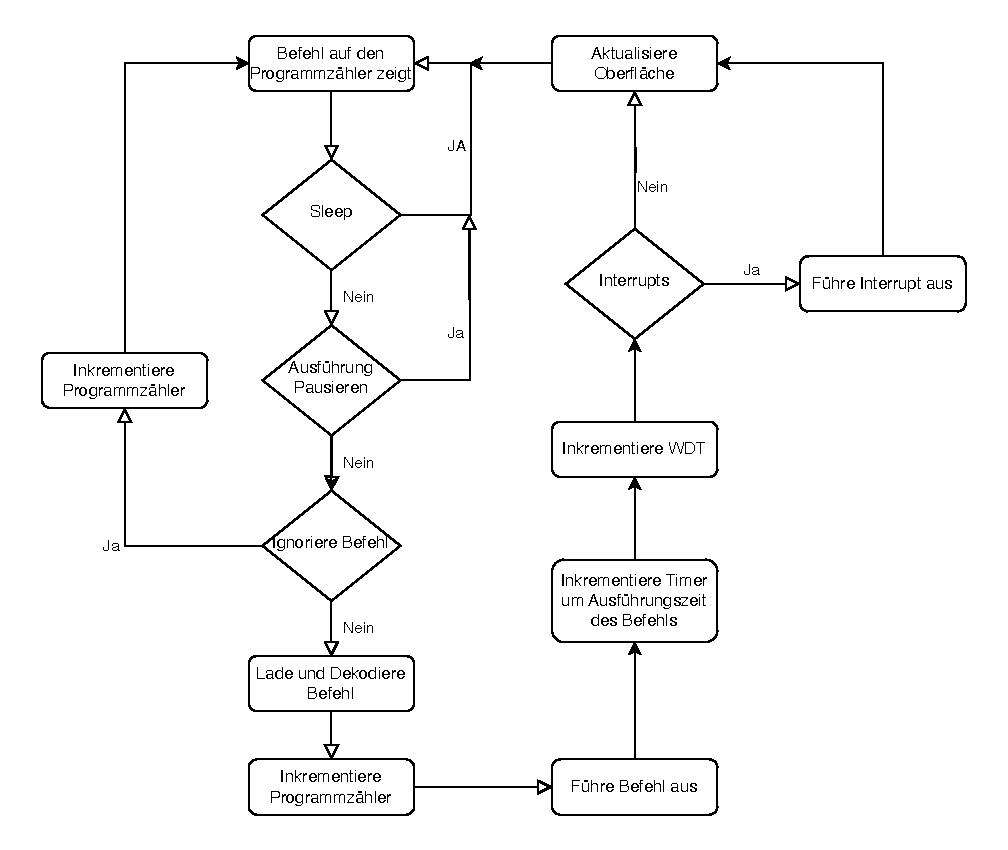
\includegraphics[width=0.9\textwidth]{./img/excec_cycle.drawio.pdf}
    \caption{Programmablauf einer Befehlsausführung}
    \label{fig:execTask}
\end{figure}


